\documentclass[10pt,a4paper,oneside]{article} % Changed to oneside for consistent alignment, not sure if we should use twoside
\usepackage[a4paper,top=20mm,bottom=20mm,outer=5cm]{geometry}
\usepackage[utf8]{inputenc}
\usepackage[english]{babel}
\usepackage{graphicx}
\usepackage{hyperref}
\usepackage{cleveref}
\usepackage{natbib}
\usepackage[table]{xcolor}
\usepackage{subcaption}
\usepackage[export]{adjustbox}

\bibliographystyle{abbrvnat}
\setcitestyle{authoryear}

\title{Project Machine Learning\\--- Milestone 1 ---} 
\author{[Imene Ben Ammar, Julian Dobler, Yannik Queisler]}
\date{\today}

\begin{document}
\maketitle

\tableofcontents
\newpage

\section{Overview}
The goal of this project is to re-implement the BERT Single Sentence Classification Model as \cite{kenton2019bert} specifies and employ it for toxic comment classification.
This report details the datasets used, feature extraction methods, baseline models, and initial baseline results .

\section{Dataset Overview}
\subsection{Data Sources}
The datasets used in this project include the SST2 Dataset used for binary classification tasks and Civil Comments and Jigsaw Toxicity Prediction Dataset used for multi-class classification tasks.
s

\subsection{Data Characteristics}
The structure of the datasets differs therefor in the hierarchy of targets, with binary labels (positive/negative) for the SST2 dataset and multiple toxicity categories, such as obscene, threat, and insult, for the Civil Comments dataset. The data distribution provides insights into the balance across these categories \textbf{[provide stats here or include image]}. The quality of the datasets was evaluated by checking for issues such as duplicates, missing values, and noise \textbf{[Did we do this?]} It was suggested to check for incomplete data and remove irrelevant entries. \textbf{[did we do this? Or write the datasets are prechecked]}

\subsection{Data Visualization}
\subsubsection{Dataset Information}
Before performing the visualization task, several key information about the datasets are displayed, in order to better understand the structure and content of the data. This includes the number of entries, column names, as well as a preview of the first few rows of each dataset.
Table \ref{Tab:dataset_info} summarizes key information about each dataset used in this project, as printed before the visualizations:
\begin{table}[h!]
\centering
\resizebox{\textwidth}{!}{%
\begin{tabular}{l|c|l}
\textbf{Dataset} & \textbf{Number of Rows} & \textbf{Columns} \\
\hline
\rowcolor{gray!10} 
Jigsaw & 223,549 & id, comment\_text, toxic, severe\_toxic, obscene, threat, insult, identity\_hate \\
Civil Comments & 1,999,514 & text, toxicity, severe\_toxicity, obscene, threat, insult, identity\_attack, sexual\_explicit \\
\rowcolor{gray!10} 
SST2 & 68,221 & idx, sentence, label \\
\end{tabular}%
}
\caption{Dataset Information}
\label{Tab:dataset_info}
\end{table}

\subsubsection{Toxicity Subtypes and Sentiment Analysis}
\begin{enumerate}
    \item Toxicity Subtypes/Sentiment Frequency: The frequency of each toxicity subtype and sentiment label was visualized using bar plots. For the toxicity subtypes, the occurrences of comments labeled as toxic for each of the subtypes were counted. For sentiment, the distribution of positive and negative labels was also plotted. This visualization provided insight into the prevalence of different types of toxicity and the overall sentiment distribution within the dataset.
    \begin{figure}[h]
    \centering
    \begin{subfigure}{0.49\textwidth}
        \centering
        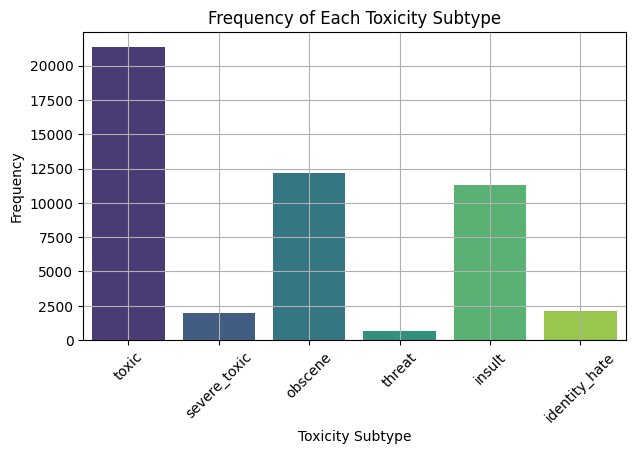
\includegraphics[width=\textwidth]{replibert/replibert/plots/Toxicity_frequency_Jigsaw.png}
        \caption{The Civil Comments dataset.}
        \label{fig:tox_freq_jigsaw}
    \end{subfigure}
    \hfill
    \begin{subfigure}{0.49\textwidth}
        \centering
        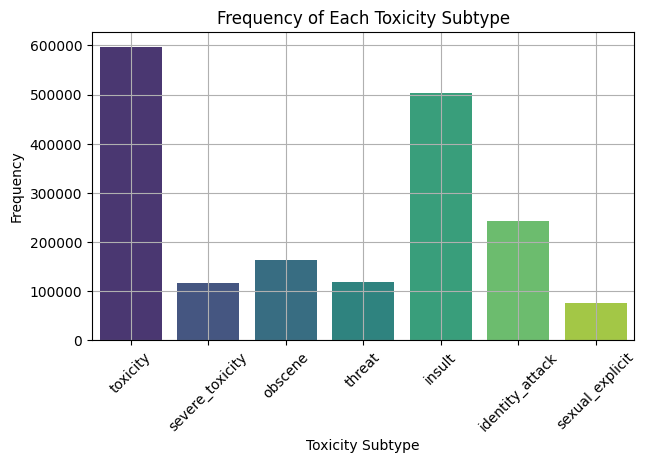
\includegraphics[width=\textwidth]{replibert/replibert/plots/Toxicity_frequency_cc.png}
        \caption{The Jigsaw\_toxicity\_pred dataset.}
        \label{fig:tox_freq_cc}
    \end{subfigure}
    \caption{Toxicity frequency plots.}
    \label{fig:tox_freq_plots}
    \end{figure}
    \item Toxicity Subtypes/Sentiment Percentage: The percentage of comments falling under each toxicity subtype and sentiment label was visualized using pie charts. The analysis considered any comment that was classified under one or more toxicity subtypes as toxic. This provided an overview of the commonness of toxic comments compared to non-toxic ones as well as positive and negative sentiments in the dataset.
    \begin{figure}[h]
    \centering
    \begin{subfigure}{0.5\textwidth}
        \centering
        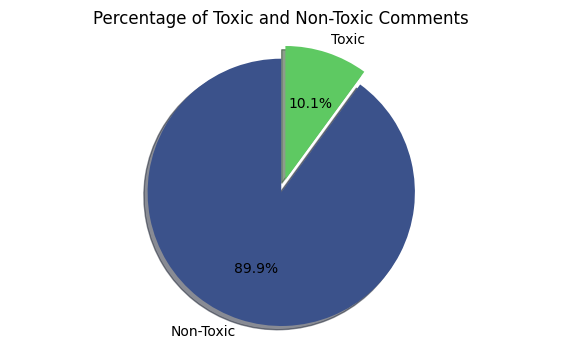
\includegraphics[width=\textwidth]{replibert/replibert/plots/Toxicity_percentage_Jigsaw.png} 
        \caption{The jigsaw\_toxicity\_pred dataset.}
        \label{fig:tox_percentage_jigsaw}
    \end{subfigure}%
    \hfill
    \begin{subfigure}{0.5\textwidth}
        \centering
        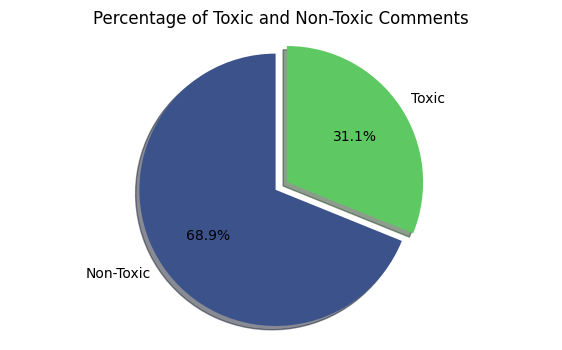
\includegraphics[width=\textwidth]{replibert/replibert/plots/Toxicity_percentage_cc.png} 
        \caption{The Civil Comments dataset.}
        \label{fig:tox_percentage_cc}
    \end{subfigure}

    \vspace{0.5cm} 
    \begin{subfigure}{0.5\textwidth}
        \centering
        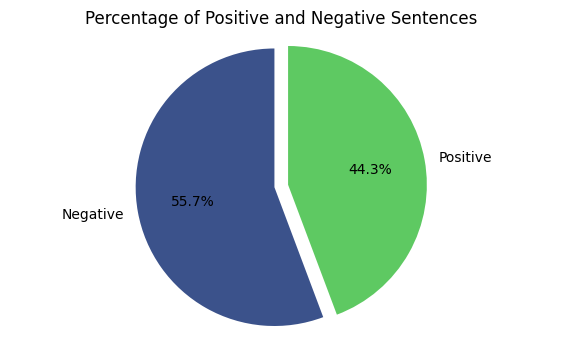
\includegraphics[width=\textwidth]{replibert/replibert/plots/sentiment_percentage.png} 
        \caption{The SST2 dataset.}
        \label{fig:sentiment_percentage}
    \end{subfigure}
    \caption{Toxicity/Sentiment percentage.}
    \label{fig:tox_sentiment_percentage}
    \end{figure}
\end{enumerate}
\subsubsection{Textual Analysis}
\begin{enumerate}
    \item Word Clouds: Seperate word clouds were generated to visually represent the most frequently occurring terms in comments labeled as toxic or non-toxic, as well as positive and negative sentiments. For the generation, again,  comments categorized as toxic included those marked with any toxicity subtype label, while sentiment labels were categorized into positive or negative. 
    \begin{figure}[h]
    \centering
    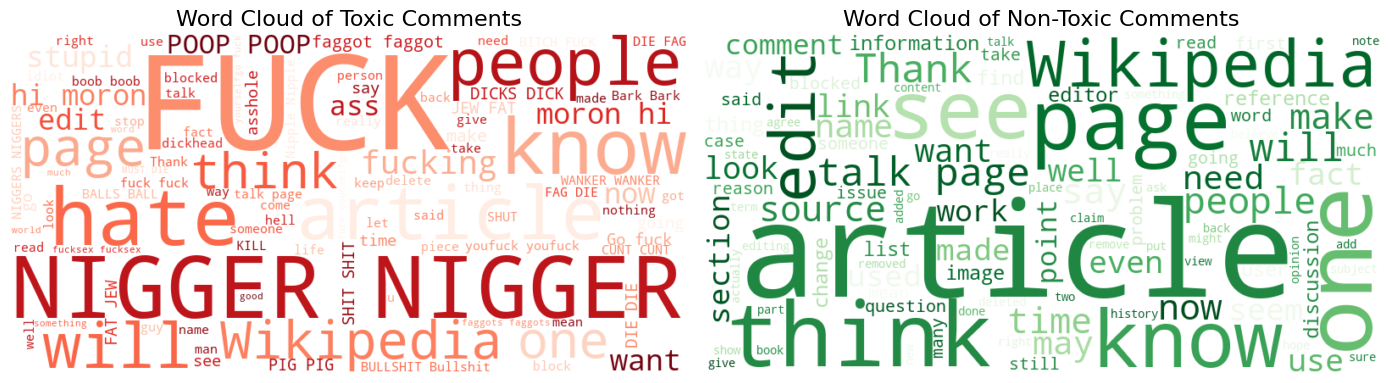
\includegraphics[width=0.9\textwidth]{replibert/replibert/plots/wordclouds_jigsaw.png}
    \caption{Example of Word Clouds for the Jisaw\_toxicity\_pred dataset.}
    \label{fig:wordcloud_jigsaw}
    \end{figure}
    \item Word Frequency: The most common words associated with \textbf{each} toxicity subtype/sentiment were identified and visualized using bar plots. As in the Civil Comments dataset, the toxicity labels are not binary but instead have continuous values to represent different degrees of toxicity, a threshold was applied to filter comments based on their toxicity score, selecting those that exceeded a threshold of 0.8. The top N (10)  most frequent words for each toxicity label/sentiment were extracted by tokenizing and cleaning the text of comments that met the threshold. The resulting word frequencies were then plotted to show the most common terms for each category. 
    \begin{figure}[h]
    \centering
    \begin{subfigure}{0.49\textwidth}
        \centering
        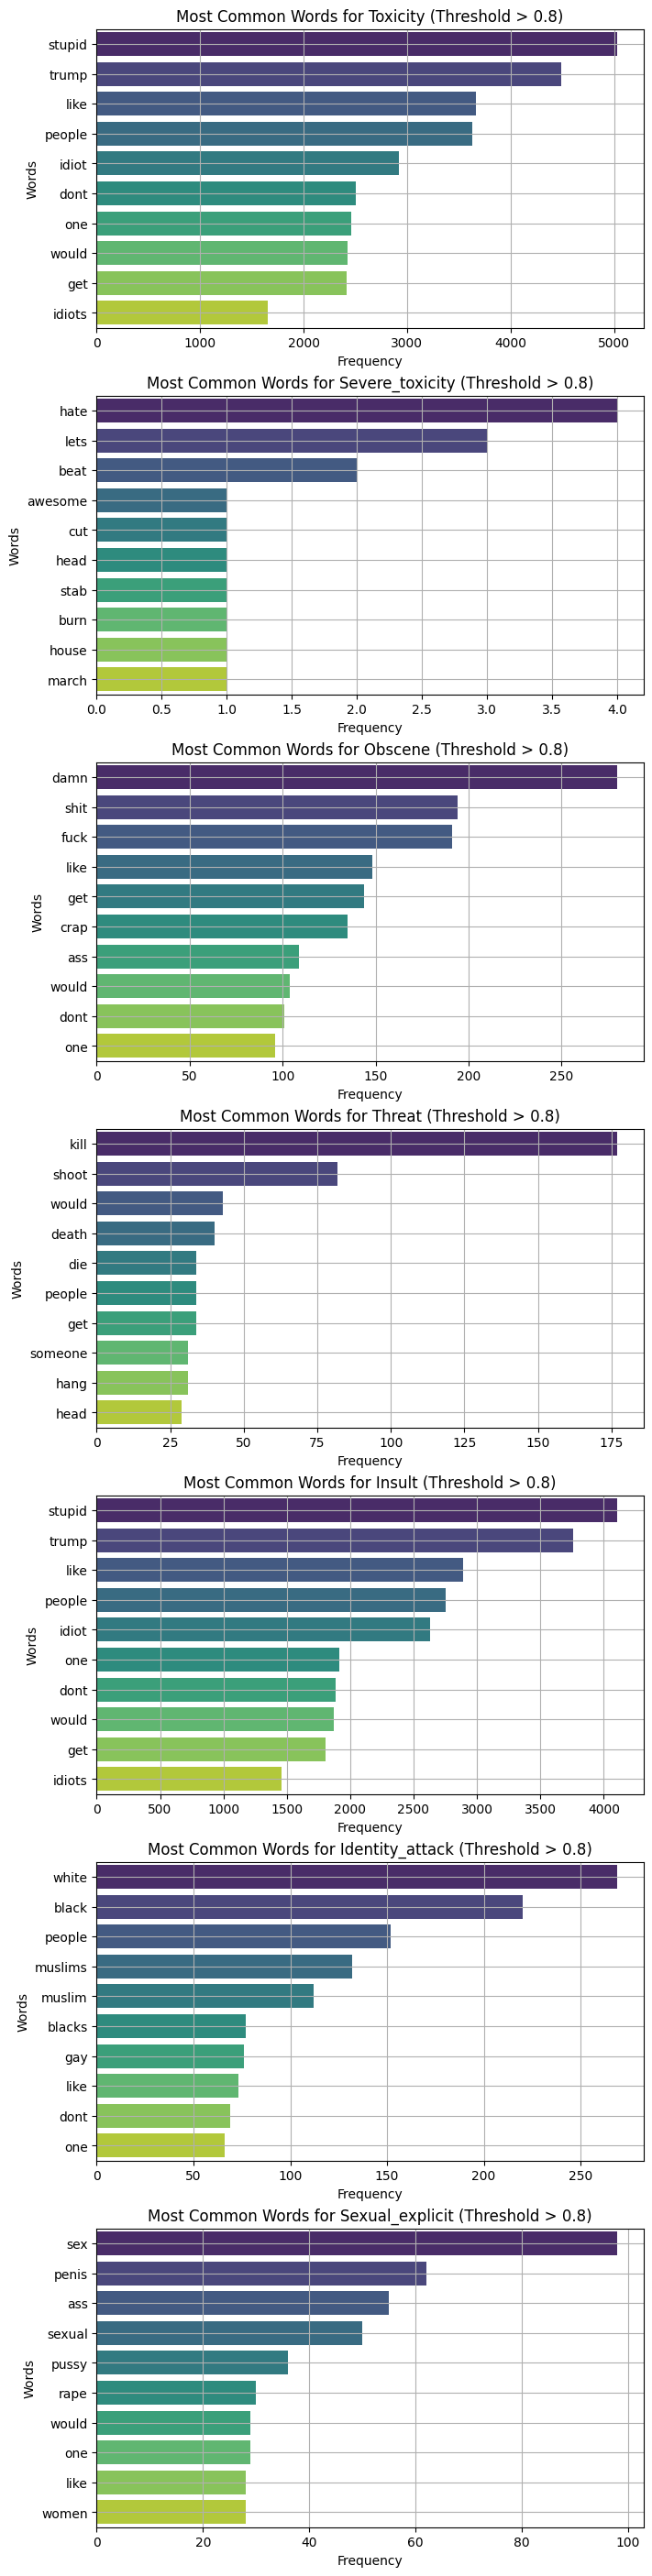
\includegraphics[width=\textwidth, clip, trim=0 290 0 1440]{replibert/replibert/plots/Word_Frequency_cc.png}
        \caption{identity\_attack subtype.}
        \label{fig:word_freq_id_attack_cc}
    \end{subfigure}%
    \hfill
    \begin{subfigure}{0.5\textwidth}
        \centering
        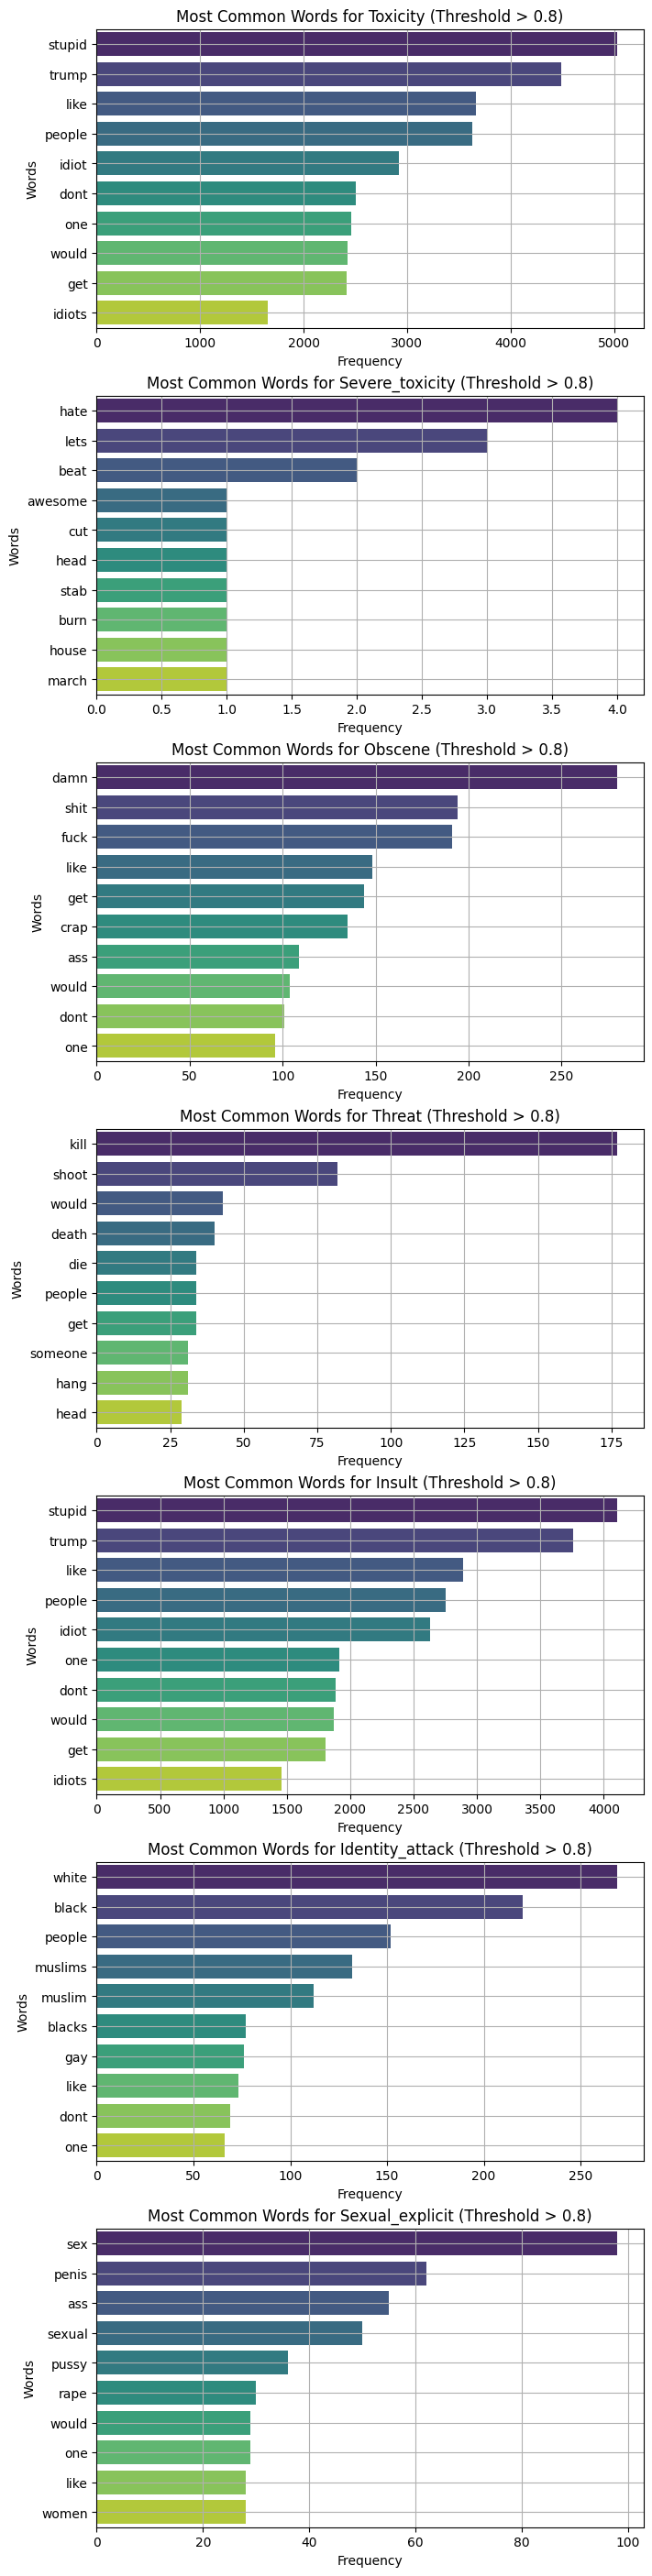
\includegraphics[width=\textwidth, clip, trim=0 870 0 870]{replibert/replibert/plots/Word_Frequency_cc.png} 
        \caption{Threat subtype.}
        \label{fig:word_freq_threat_cc}
    \end{subfigure}
    \caption{Example of word frequency plots for the Civil Comments datasets for two toxicity subtypes.}
    \label{fig:word_freq_cc}
    \end{figure}
    \item Comment Length: In order to identify potential patterns between comment length and toxicity/sentiment in the datasets, the lengths of comments in all datasets were analyzed. This included plotting histograms of the distribution of comment lengths, box plots to highlight the differences in comment length across the different categories (Toxic vs. Non Toxic and Positive vs. Negative), and bar plots to illustrate the average comment lengths per category. 
    \begin{figure}[h]
    \centering
    \begin{subfigure}{0.5\textwidth}
        \centering
        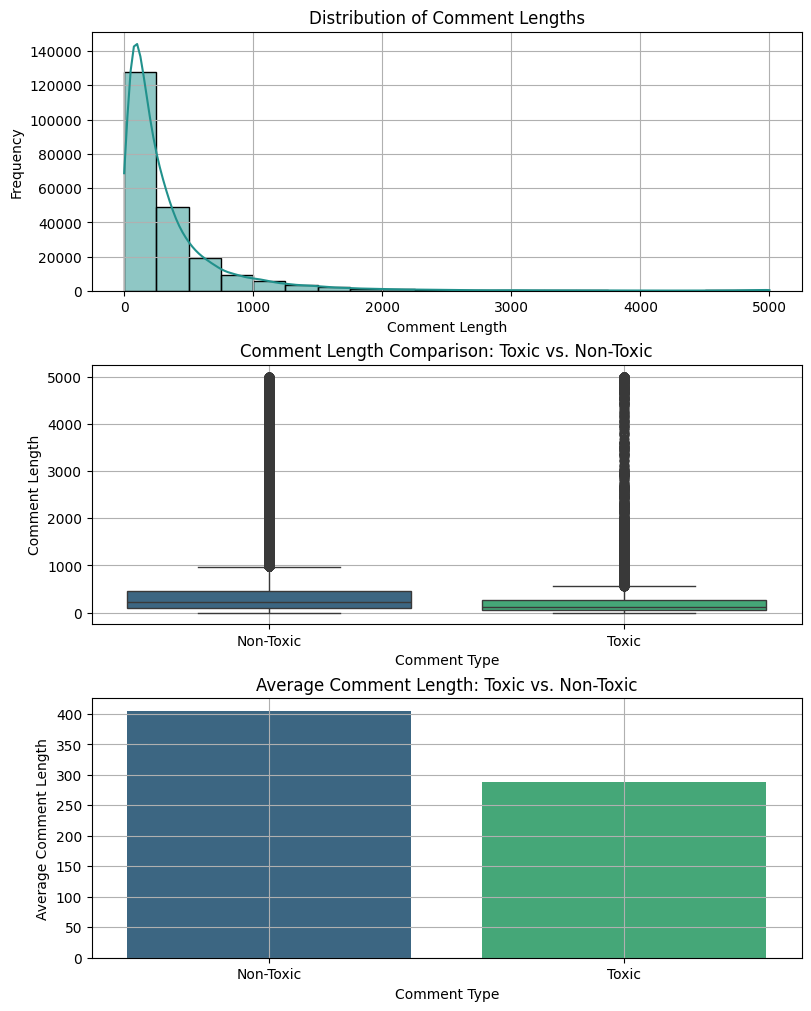
\includegraphics[width=\textwidth, clip, trim=0 240 0 730]{replibert/replibert/plots/comment_len_jigsaw.png}
        \vspace{6em}
        \caption{The jigsaw\_toxicity\_pred dataset.}
        \label{fig:comment_len_jigsaw}
    \end{subfigure}%
    \hfill
    \begin{subfigure}{0.5\textwidth}
        \centering
        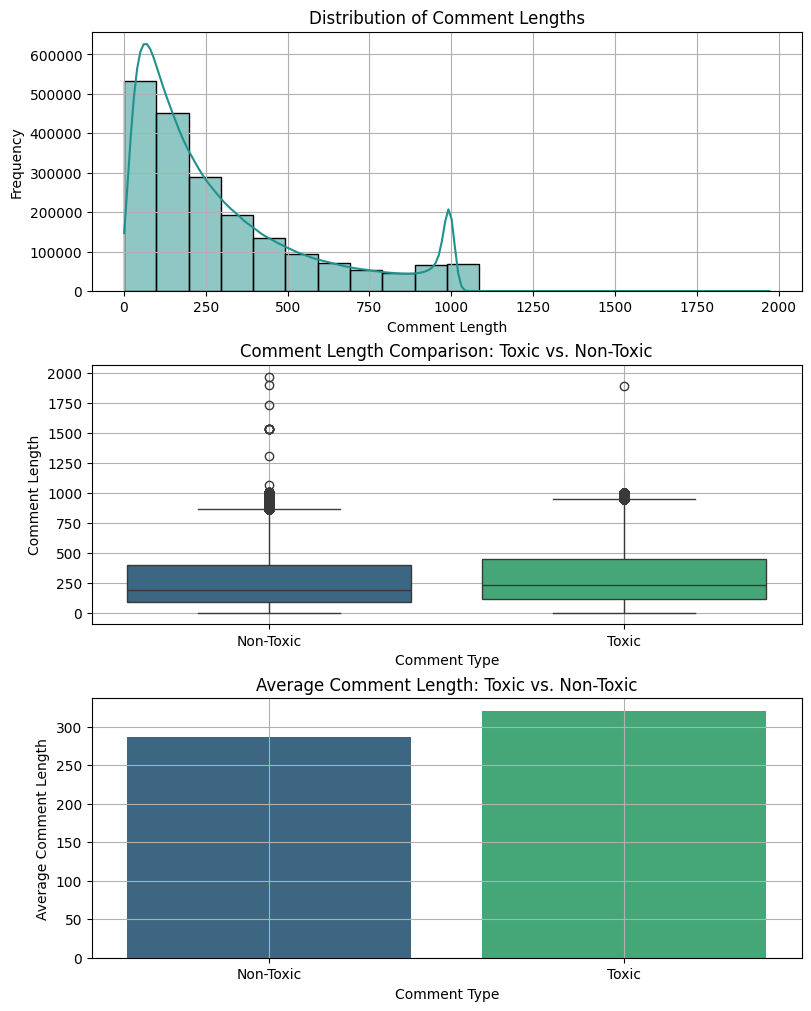
\includegraphics[width=\textwidth, clip, trim=0 240 0 730]{replibert/replibert/plots/comment_len_cc.png} 
        \vspace{6em}
        \caption{The Civil Comments dataset.}
        \label{fig:comment_len_cc}
    \end{subfigure}
    \caption{Average comment length.}
    \label{fig:comment_len_plots}
    \end{figure}
    \item Toxicity Subtypes vs. Comment Length: Scatter plots were created to explore the relationship between comment length and various toxicity subtypes in the Jigsaw and Civil Comments datasets. For each toxicity label, a scatter plot was generated with comment length on the x-axis and the toxicity level on the y-axis. These plots allow for the visualization of potential correlations between the length of comments and the increase of toxicity level and therefore provide insights into whether longer comments tend to be more toxic or if there is no clear relationship between comment length and toxicity. This plot is more useful in the Civil Comments datasets, as the toxicity values are not binary. 
    \begin{figure}[h]
    \centering
    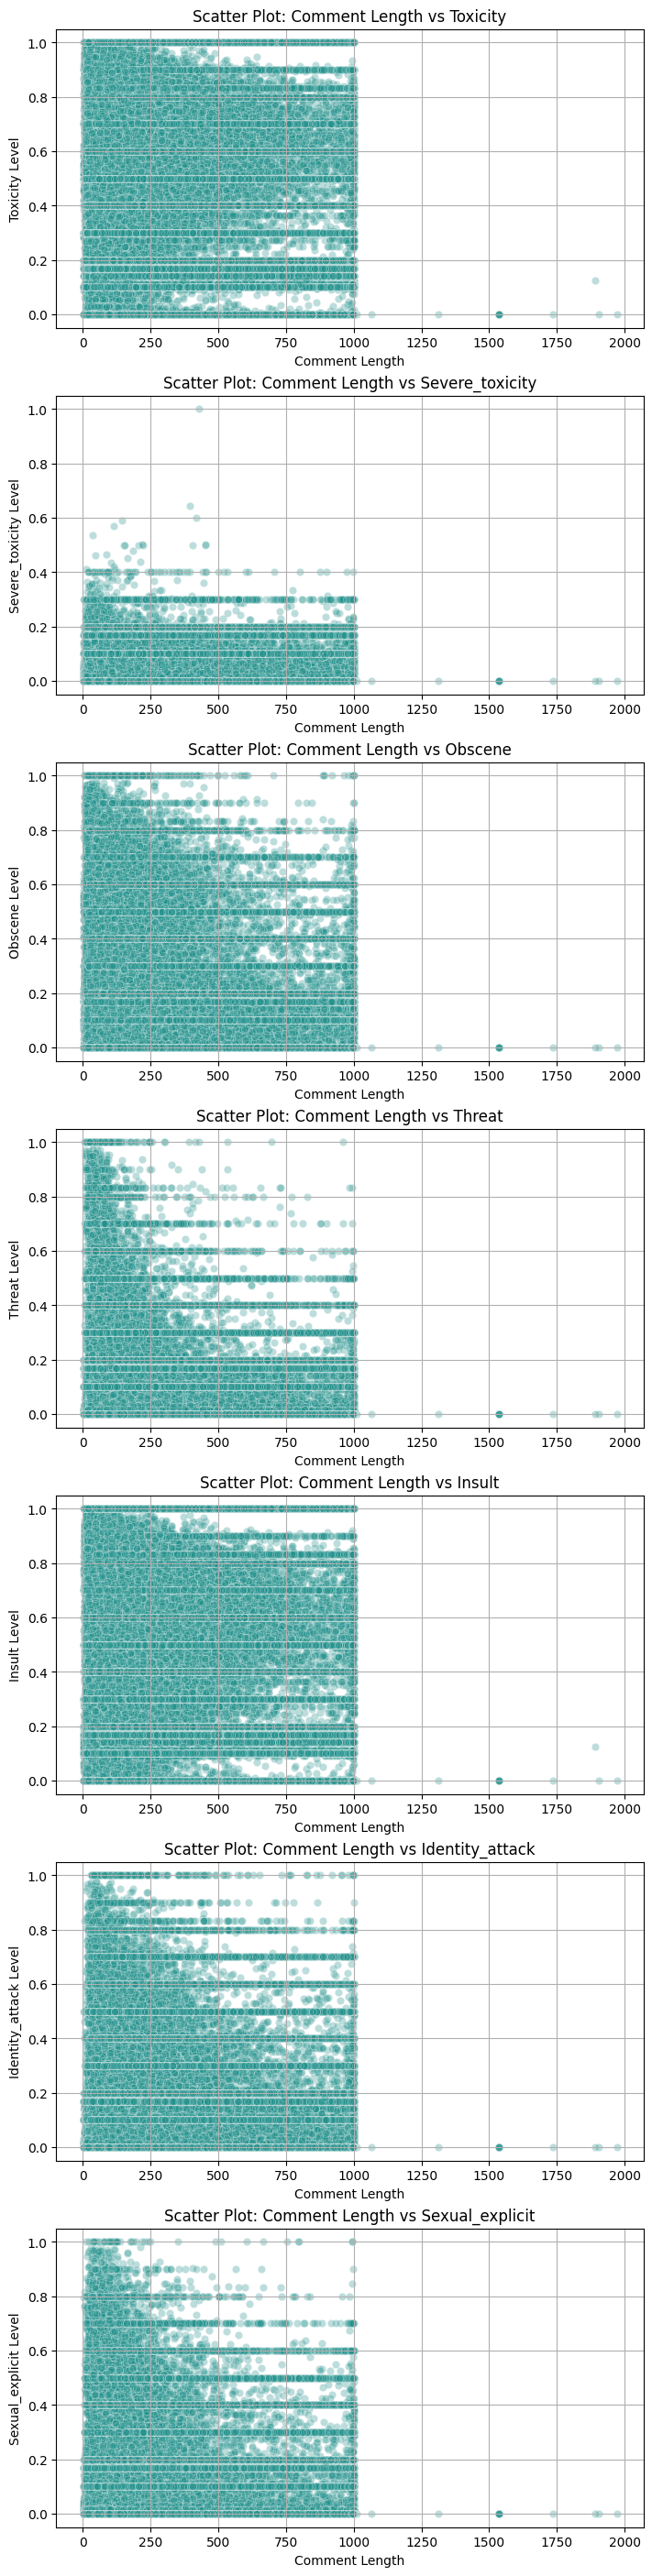
\includegraphics[width=0.8\textwidth,clip,trim=0 865 0 865.5]{replibert/replibert/plots/toxicity_length_cc.png}
    \caption{Toxicity subtype vs. comment length example for the Civil Comments dataset.}
    \label{fig:tox_vs_len_cc}
    \end{figure}
\end{enumerate}
All previous plots can be done by running the \texttt{show()} function which loads the dataset from the disk based on the provided \texttt{dataset} name (\texttt{'Jigsaw'}, \texttt{'civil\_ comments'} or \texttt{'SST2'}), selects and executes the appropriate plotting function based on the \texttt{plot\_type (e.g., toxicity\_frequency, sentiment\_percentage...)} and dataset parameters provided. Optionally the generated plot is saved to a file (\texttt{outfile}) if provided and displayed.
\subsection{Feature Extraction}
We apply the BERT model and the baseline models on the datasets. These models need different features, therefore we identify two feature extraction methods which can be used on the raw dataset. We also implement the function \texttt{load\_data} which provides data in the required format.
\subsubsection{BERT Feature Extraction}
For the BERT model, feature extraction is based on the BERT tokenizer, which converts text into token IDs. BERT embeddings incorporate word, position, and token type embeddings, as described in \cite{kenton2019bert}. 
\subsubsection{Baseline Feature Extraction}
For the baseline methods we use TF-IDF (Term Frequency-Inverse Document Frequency) features. These are used for the Bayesian and logistic regression baseline methods because they effectively quantify the importance of words in a document relative to the entire dataset. TF-IDF assigns higher weights to words that appear frequently in a specific document but less frequently across the corpus, helping to filter out common stop words and focus on terms that are more relevant the the meaning of the specific document \citep{sparck1972statistical}. This makes TF-IDF appropriate for text classification tasks, as it provides a simple and rich representation of textual data that can be used as input of machine learning models like Naive Bayes and logistic regression.
\subsubsection{Loading Data}
As part of our data pipeline, we implement the function \texttt{load\_data}. This function is designed to support various feature extraction techniques by accepting a transformation argument that specifies the desired feature extractor. For the BERT model, the transformation utilizes the BERT tokenizer.  For baseline models like Naive Bayes and logistic regression, the transformation would be the TF-IDF feature extractor. By leveraging this modular design, the \verb|load_data| function ensures flexibility and compatibility with different approaches.
\textbf{[Missing: feature normalizing?, different shape inputs,  answers by ML about data ]}

\section{Baseline Method and Evaluation}
\subsection{Baseline Models}

We applied two baseline models in this porject, inlcuding Naive Bayes and Logistic Regression. Each is well suited for the dataset it is employed on. 
\subsubsection{Naive Bayes}
Naive Bayes was applied to the SST2 dataset for binary classification.  This algorithm levereges knowledge about the probability of features appearing in each class. It then classifies a given sample based on its features under the assumption of probabilistic independence of the different features. 
\subsubsection{Logistic Regression}
 Logistic regression, on the other hand, was employed on the Civil Comments and Jigsaw Toxicity datasets, which involve multi-class classification. This algorithm predicts the probability of an instance belonging to a class by applying a sigmoid function to a linear combination of input features. 
 
 \textbf{[Add why we use different models for the two tasks]}
\subsection{Evaluation Metrics}
\begin{itemize}
    \item \textbf{[provide eval metric for binary-class classification]}
    \item \textbf{[provide eval metri for multi-class classification]}
\end{itemize}

\subsection{Results}
\begin{itemize}
    \item \textbf{Naive Bayes (SST2):} [provide results]
    \item \textbf{Logistic Regression (Civil Comments and Jigsaw):} [provide results]
\end{itemize}

\subsection{Overfitting and Challenges}
\begin{itemize}
    \item \textbf{[Did we do anything against overfitting?]}
    \item \textbf{[Different categories characterization?]}
    \item \textbf{[Something non-techincal about good features]}

\end{itemize}


\section{Discussion}
\subsection{Key Insights}
\begin{itemize}
    \item \textbf{[what are challenges of the datasets]}
    \item \textbf{[why is task not trivial]}
    \item \textbf{[why is answer from model interesting]}

\end{itemize}

\subsection{Future Directions}
\begin{itemize}
    \item \textbf{[What does or doesn't work, why?]}
    \item \textbf{[what is possible with the datasets, usuful in business?]}
    \item \textbf{[things we want to try]}
\end{itemize}



\bibliography{report_template}
\end{document}